\section{Lezione 19}

Facciamo alcuni esempi di architetture software. Il progettista fissa quanti livelli servono e le interfacce che interagiscono tra questi livelli. Fissa una regola di dialogo sui livelli in modo da avere interazioni utili. Dentro ciascuna scatola le informazioni sono completamente incapsulate.

\begin{center}
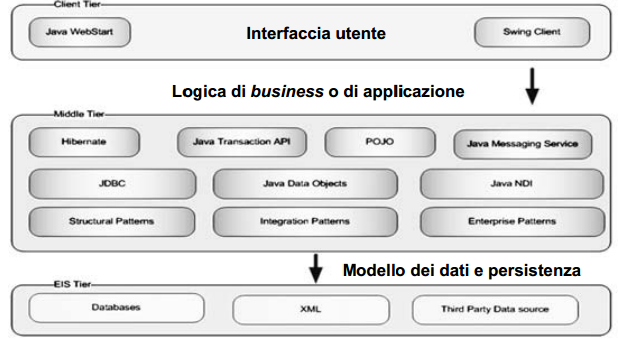
\includegraphics[width=0.75\columnwidth]{img1} % Example image
\end{center}

Tra l'interfaccia utente ed il modello dei dati c'� un supporto a specifiche procedure che forniscono la logica d'applicazione. Si vorrebbe scrivere una logica applicativa che non dipenda dalla base dati specifica, e questa cosa ce la fornisce il \textbf{framework}.

Architettura di relazione, \textbf{MVC-2}.

\begin{center}
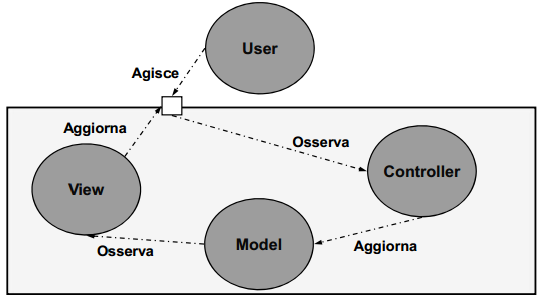
\includegraphics[width=0.75\columnwidth]{img2} % Example image
\end{center}

L'errore grande che si pu� fare � quello di pensare di fare una documentazione non tecnica o narrativa. Scriveremo testi basati su una sequenza di diagrammi e poche frasi di collegamento. Questo documento ha un suo linguaggio. Per \textbf{componente} si intende un elemento dell'architettura con delle interfacce chiare e formate. Relazioni tra pi� componenti espresse con delle frecce. Una \textbf{parte} � un'interfaccia esposta da una componente architetturale. Un \textbf{connettore} � una conenessione tra pi� parti (in UML si chiama \textit{associazione}). � importante capire che l'architettura dev'essere valutata per la sua \textbf{qualit�}. Cercheremo metodi utili e ambienti di progettazione che questi metodi importano. Questo perch� perseguiamo \textit{qualit� by construction}. Vogliamo che la \textbf{baseline} sia pulita e quindi bisogna verificare che l'architettura lo sia. La progettazione la distingueremo in due fasi (lassi di tempo contigui e continui):

\begin{itemize}

	\item Una di \textbf{alto livello} in cui fissiamo l'architettura e i pattern;
	\item Una di \textbf{dettaglio} in cui riempiamo i buchi per agevolare il lavoro del programmatore. Progettare parti piccole che chiameremo \textbf{moduli}.

\end{itemize}

Al progettista chiediamo di garantire che la sua attivit� sia funzionale. Un \textbf{modulo} � un'unit� di lavoro che � utile ed opportuno affidare ad un singolo programmatore. Una classe troppo grossa non va bene, sbilancia il lavoro. Voglio un insieme di caratteristiche che stiano bene insieme. Finch� non ho ridotto le classi a modulo non posso partire con la programmazione. Se ho classi molto modulari posso far lavorare pi� programmatori in parallelo.

Per descrivere l'architettura serve un \textbf{documento}, per produrre questo possiamo riferirci a degli standard procedurali, i quali sono per� troppo rigidi. Si � capito che non � utile imporre procedure. Non � formativo imporre strutture di documenti, ma produrre processi. A noi interessa chiederci che cosa dobbiamo raccontare rispetto alle attese del committente. I documenti non devono avere una struttura standard.

\textbf{Stati di processo} per SEMAT:

\begin{itemize}

	\item \textbf{Architecture selected}: dobbiamo scegliere l'architettura e dobbiamo spiegare perch� essa � adatta al sistema. Selezione delle tecnologie necessarie, posso quindi fare stime di costo sensate. Decisione su \textbf{buy}, \textbf{build}, \textbf{make}. In questo stadio di avanzamento non c'� nemmeno una linea di codice, niente di realizzato;
	\item \textbf{Demonstrable}: dimostrazione delle principali caratteristiche del sistema agli stakeholder, i quali concordano. Decisioni su interfacce e configurazioni di sistema. Ho fatto e ho completato la progettazione ad alto livello ed eventualmente ho dei prototipi, ma non ho ancora implementato nulla;
	\item \textbf{Usable}: il sistema � usabile e ha le caratteristiche desiderate. Non � completamente finito, ho ancora difetti, ma essi sono accettabili. Quindi possiamo \textit{sperare} di iniziare a fare la revisione di collaudo;
	\item \textbf{Ready}: il prodotto � cos� maturo che posso iniziare a scrivere il \textbf{manuale utente}. Si � infatti professionali se si fornisce all'utente un manuale con una struttura. E in quest'epoca non sono pi� solo documenti cartacei, ma anche e soprattutto con altri mezzi.

\end{itemize}

``La documentazione � l'incubo dei cowboy''. La documentazione deve essere una conseguenza dei processi organizzativi. Le attivit� che svolgo devono produrre tutto o quasi tutto. Serve documentare nel modo meno intrusivo possibile. Fra le cose pi� importanti che fa la documentazione � fornire una misura sull'avanzamento del progetto (Piano di progetto), che fornisce dei \textbf{consuntivi} (stato fotografato) e \textbf{preventivi} (stime). I consuntivi sono finali se siamo alla fine del progetto, o parziali se siamo in corso. � bene misurare solo le cose utili e interessanti. Misureremo le cose sulle quali possiamo e vogliamo fissare degli obiettivi di miglioramento. Vorrei misurare per esempio quante volte modifico i requisiti. Misurazione per obiettivi. 

Il responsabile di progetto deve avere un ``\textit{cruscotto}'' con gli indicatori delle metriche che utilizziamo, e questi indicatori devono essere aggiornati. Vogliamo inoltre che il responsabile spenda il meno possibile. Voglio documentare tutte le attivit� di pianificazione, gestione, sviluppo, verifica e validazione. In poche parole dobbiamo documentare \textbf{tutto}. Il piano ci d� degli obiettivi sui tempi e costi, le norme sono invece gli strumenti e le procedure che uso per rendere il piano fattibile. Il primo e pi� importante documento da realizzare (interno) sono le \textbf{norme di progetto}, che cresceranno nel tempo. Una volta che ho le norme posso pensare al piano. Questi non sono documenti di progettazione, analisi o verifica.

Ogni architettura software ha molte viste:

\begin{itemize}

	\item \textbf{Modello statico}, inteso come componenti, ``quali sono le cose'', come si relazionano;
	\item \textbf{Modello dinamico}, come le parti interagiscono tra di loro;
	\item \textbf{Modello delle interfacce};
	\item \textbf{Modello delle relazioni}, quali dati fluiscono tra i componenti;
	\item \textbf{Modello di distribuzione}, associazione tra nodi fisici e componenti logiche.

\end{itemize}

L'architettura va descritta in due documenti distinti:

\begin{itemize}

	\item \textbf{Specifica tecnica};
	\item \textbf{Definizione di prodotto}: ho bisogno di una \textit{milestone} che dica che questa � una buona architettura.

\end{itemize}

Architettura della documentazione:

\begin{center}
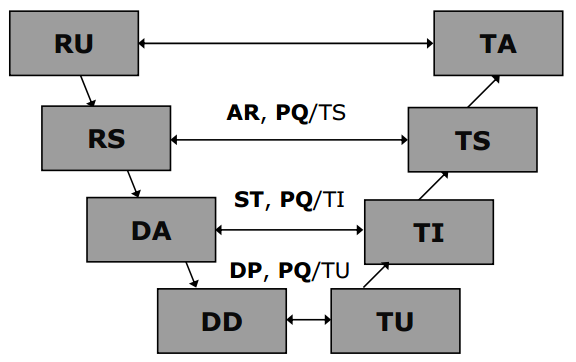
\includegraphics[width=0.75\columnwidth]{img3} % Example image
\end{center}